\documentclass[11pt]{article}
\usepackage[english,russian]{babel}
\usepackage{url}
%для поддержки русского
\usepackage{graphicx,DCCN2019_ru}
%пакет с нужными мне штуками
%для красивых символов
\usepackage{upgreek}
\usepackage{dsfont}
\usepackage{amssymb}
\usepackage{tipa}
\usepackage{ wasysym }
\usepackage{gensymb} %градусы
%зачеркивание текста
\usepackage{cancel}
%для цветного текста
\usepackage[usenames]{color}
%для ссылок
\usepackage{xcolor}
\usepackage{hyperref}
% Цвета для гиперссылок
\definecolor{linkcolor}{HTML}{0000ff} % цвет ссылок
\definecolor{urlcolor}{HTML}{0000ff} % цвет гиперссылок
\hypersetup{pdfstartview=FitH,  linkcolor=linkcolor,urlcolor=urlcolor, colorlinks=true}
%Для вставки картинок
\graphicspath{{pictures/}}
\DeclareGraphicsExtensions{.pdf,.png,.jpg}

%команды
\usepackage{amsmath,amsthm,amssymb,amsfonts, enumitem, fancyhdr, color, comment, graphicx, environ}

%настройки текста
\pagestyle{fancy} 
\fancyhead{} 
\fancyfoot{} 
\usepackage[utf8]{inputenc}

%настройки страницы
\makeatletter
\fancyhead[R]{\small Павел Костин}
\fancyhead[L]{\small Матмех СПбГУ}
\fancyhead[C]{\small Билеты, мат. анализ, 2 семестр, 2019}
\pagestyle{fancy}
\fancyfoot[R]{\thepage}

%команды
\usepackage{amsmath,amsthm,amssymb,amsfonts, enumitem, fancyhdr, color, comment, graphicx, environ}
%римские цифры
\newcommand{\RNumb}[1]{\uppercase\expandafter{\romannumeral #1\relax}}
%команды для ускорения набора
\newcommand{\R}{\mathds{R}}
\newcommand{\Q}{\mathds{Q}}
\newcommand{\Z}{\mathbb{Z}}
\newcommand{\B}{\mathcal{B}}
\newcommand{\CC}{\mathds{C}}
\newcommand{\N}{\mathds{N}}
\newcommand{\ra}{\Rightarrow}
\newcommand{\la}{\Leftarrow}
\newcommand{\rla}{\Leftrightarrow}
\newcommand{\lra}{\Leftrightarrow}
\newcommand{\e}{\exists}
\newcommand{\E}{\mathcal{E}}
\newcommand{\q}{\quad}
\newcommand{\devides}{\mathop{\raisebox{-2pt}{\vdots}}}

%вёрстка
\newenvironment{solutions}[1][]
{\begin{trivlist}\item{\underline{\bfseries #1}}}{\end{trivlist}\newpage}
\newenvironment{definition}[1][Опр.]
{\begin{trivlist}\item{\underline{\bfseries #1} }}{\end{trivlist}}
\newenvironment{definition2}[2][Опр]
{\begin{trivlist}\item[\underline{{\bfseries #1}} {\bfseries #2.}]}{\end{trivlist}}
\newenvironment{instance}[1][Пример.]
{\begin{trivlist}\item{\underline{\bfseries #1} }}{\end{trivlist}}
\newenvironment{instances}[1][Примеры.]
{\begin{trivlist}\item{\underline{\bfseries #1} }}{\end{trivlist}}
\newenvironment{statement}[1][Утв.]
{\begin{trivlist}\item{\underline{\bfseries #1} }}{\end{trivlist}}
\newenvironment{lemma}[1][Лемма.]
{\begin{trivlist}\item{\underline{\bfseries #1} }}{\end{trivlist}}
\newenvironment{lemma2}[2][Лемма]
{\begin{trivlist}\item[\underline{{\bfseries #1}} {\bfseries #2.}] \hspace{0pt} \\}{\end{trivlist}}
\newenvironment{comments}[1][Замечание.]
{\begin{trivlist}\item{\underline{\bfseries #1} }}{\end{trivlist}}
\newenvironment{theorem}[1][Теорема.]
{\begin{trivlist}\item{\underline{\bfseries #1} }}{\end{trivlist}}
\newenvironment{theorem2}[2][Теорема]
{\begin{trivlist}\item[\underline{{\bfseries #1}} {\bfseries #2.}] \hspace{0pt} \\}{\end{trivlist}}
\newenvironment{reminder}[2][Напоминание]
{\begin{trivlist}\item[\underline{{\bfseries #1}} {\bfseries #2:}] \hspace{0pt} \\}{\end{trivlist}}
\newenvironment{proofs}[1][Доказательство.]
{\begin{trivlist}\item{\bfseries #1} }{\end{trivlist}}
\newenvironment{proofs2}[2][Доказательство]
{\begin{trivlist}\item[\underline{{\bfseries #1}} {\bfseries #2.}]\hspace{0pt}} {\end{trivlist}}
\newenvironment{proofByDisagreement}[1][Доказательство (от противного). ]
{\begin{trivlist}\item{\bfseries #1}}{\end{trivlist}}
\newenvironment{proofByInduction}[1][Доказательство (по индукции). ]
{\begin{trivlist}\item{\bfseries #1}}{\end{trivlist}}
\newenvironment{properties}[1][Свойство.]
{\begin{trivlist}\item{\underline{\bfseries #1} }}{\end{trivlist}}
\newenvironment{properties2}[2][Свойства]
{\begin{trivlist}\item[\underline{{\bfseries #1}} {\bfseries #2.}]\hspace{0pt}} {\end{trivlist}}
\newenvironment{consequence}[1][Cледствие.]
{\begin{trivlist}\item{\underline{\bfseries #1} }}{\end{trivlist}}
\newenvironment{consequence2}[2][Cледствие]
{\begin{trivlist}\item[\underline{\bfseries #1} {\bfseries #2.}]}{\end{trivlist}}

%фикс отступа
\usepackage{tocloft}
\setlength{\cftbeforetoctitleskip}{1em}

%сам документ
\begin{document}
\begin{center}
  \huge Лекции по алгебре
  
  (читает Роткевич А. С.)
\end{center}
Данный документ неидеальный, прошу сообщать о найденных недочетах в \href{https://vk.com/drab_existence_a}{вк}
\tableofcontents
\newpage

%билеты
\section{Функции от нескольких переменных}
\subsection{02.09.2019}

\begin{definition}
    $\rho: X * X \rightarrow \R$ - метрика, если
    \begin{enumerate}                               
    	\item $\rho(x,y) \geqslant 0$, $\rho(x,y)=0 \Leftrightarrow x=y$
    	\item $\rho(x,y)=\rho(y,x)$
    	\item $\rho(x,y) \leqslant \rho(x,z)+\rho(z,y)$
    	
    	$(X,\rho)$ - метрическое пространство
	\end{enumerate} 
\end{definition}

\begin{instances}
    \begin{enumerate}  
        \item $\R$ $\rho(x,y)=|x-y|$
        \item $x \neq \varnothing$ $\rho(x,y)=
            \begin{cases}
                1, \q x \neq y\\
                0, \q x=y
            \end{cases}$
        \item $\R^n$, $n \geqslant 1$ $\rho(x,y)=\sqrt{(x_1-y_1)^2+...+(x_n-y_n)^2}$, где $x=(x_1,...,x_n)$ $y=(y_1,...,y_n)$
    \end{enumerate} 
\end{instances}

\begin{definition}
    $\rho_1, \rho_2: X*X \rightarrow \R$ - метрики, тогда $\rho_1, \rho_2$ - эквивалентны, если (они задают одну топологию) $с_1 \rho_1 (x,y) \leqslant \rho_2 (x,y) \leqslant c_2 \rho_1(x,y)$ для $c_1,c_2>0$ - const
\end{definition}

\begin{instance}
    $\R^2$ $\rho_1(x,y) = \sqrt{(x_1-y_1)^2 + (x_2-y_2)^2} \leqslant \sqrt{2 \rho_2^2(x,y)}$
    
    $\rho_2(x,y)=max(|x_1-y_1|, |x_2-y_2|)$ (упр.)
    
    $\frac{1}{\sqrt{2}} \rho_1(x,y) \leqslant \rho_2(x,y) \leqslant \rho_1(x,y)$
    
    Пусть $\rho_3(x,y)=(|x_1-y_1|^p+...|x-n-y_n|^p)^{\frac{1}{p}}$, $p \geqslant 1$
    
    Если $p \rightarrow \infty$ $\rho_3 \rightarrow \rho_2$
    
    $l_n^p=(\R^n,\rho_3)$ - пространство Лебега конечномерное
    
    (упр.) Д-ть, что все метрики эквивалентны $(\rho_1,\rho_2,\rho_3)$
\end{instance}
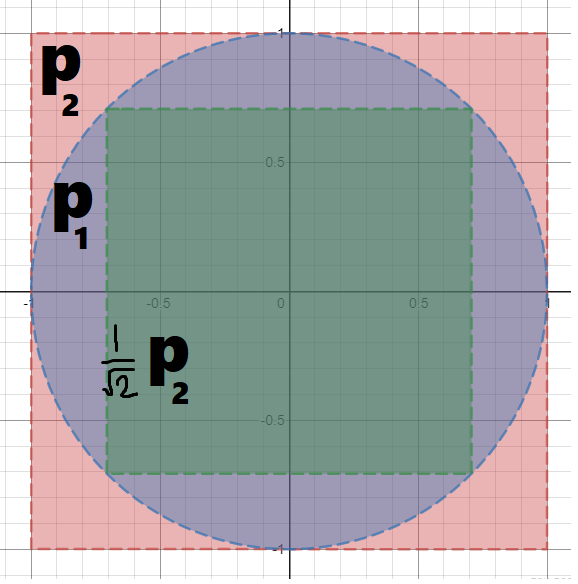
\includegraphics[scale=0.3]{pictures/p1p2p3.png}

\begin{definition}
    $\rho: X*X \rightarrow \R$ - метрика, 
    
    Открытым шаром в X относительно метрики $\rho$ называется мн-во $B_r(x)=B(x,r)=\{y \in X: \rho(x,y) < r \}$
    
    Замкнутым шаром называется $\overline{B}_r(x)=\{y \in X: \rho(y,x) \leqslant r \}$
    
    Сферой называется $S_r(x)=\{y \in X: \rho(x,y)=r \}$
\end{definition}

\begin{exercise}
    Замкнутый шар - не всегда замыкание шара (см. дискретную метрику)
\end{exercise}

\begin{instance}
    $l^p=\{ \{x_n\}_{n=1}^\infty: \sum\limits_{n=1}^\infty |x_n|^p < \infty \}$ $1 \leqslant p < \infty$
    
    $\rho(\{x_n\}_{n=1}^\infty, \{y_n\}_{n=1}^\infty) = (\sum\limits_{n=1}^\infty (x_n-y_n)^p)^{\frac{1}{p}}$
    
    $l^p$ - пр-во Лебега (последовательностей)
\end{instance}

\begin{instance}
    $C[0,1]$ - пр-во непр. функций
    
    $\rho(f,g)=\max\limits_{[0,1]} |f-g|$ - полна (любая фундаментальная последовательность сходится)
    
    $\rho_p(f,g)=(\int\limits_0^1 |f-g|^p dx)^{\frac{1}{p}}$ - не полная
\end{instance}

\begin{definition}
    $(X, \rho)$ - метр. пр-во, $\{x_k\}_{k=1}^\infty \subset X$, $a \in X$ $x_k \rightarrow a$ в пр-ве X по метрике $\rho$, если $\rho(x_n,a) \underset{k \rightarrow \infty}{\rightarrow} 0$
\end{definition}

\begin{instances}
    $\R^2$ $M_k=(x_k, y_k)$ $P=(a,b)$ $M_k \rightarrow P$ в евкл. метрике, т.е. $\rho(M_k,P)=\sqrt{(x_k-a)^2+(y_k-b)^2} \underset{k \rightarrow \infty}{\rightarrow} 0 \lra x_k \rightarrow a,\ y_k \rightarrow b$
\end{instances}

\begin{comments}
    Есть $\rho_1,\rho_2$ - экв. метрики, то $\rho_1(x_k,a) \rightarrow 0 \lra \rho_2(x_k,a) \rightarrow 0$
\end{comments}

\begin{exercise}
    $x_k \rightarrow a,\ x_k \rightarrow b \ra a=b$
    
    ($\rho(a,b) \leqslant \rho(a, x_k) + \rho(x_k,b) \rightarrow 0 \ra \rho (a,b) \rightarrow 0 \ra a=b$)
\end{exercise}

\begin{definition}
    $E \subset X$, $(X, \rho)$ - метр. пр-во, $a \in X$ - т. сгущ. E, если $\forall \E \ \e x \in E: \rho(a,x) < \E$
\end{definition}

\begin{definition}
    $f:E \rightarrow Y$ $(X, \rho)$, $(Y,d)$ - метр. пр-ва $(E \subset X)$, а - т. сгущ. E, $A \in Y$, тогда A - предел отображения f в т. а, если $f(x) \rightarrow A$ при $x \in E \setminus \{a\}\rightarrow a$\\
    (или $\forall \E>0 \q \e \delta>0: \rho(x,a)<\delta$ и $x \in E \subset \{a\}$, то $d(f(x),A) < \E)$\\
    Обозначение: $A=\lim\limits_{x \rightarrow a} f(x)$ или $f(x) \rightarrow A$ $x \rightarrow a$
\end{definition}

\begin{comments}
    $A=\lim\limits_{x \rightarrow a} f(x) \lra \forall \E > 0 \ \e \delta>0: f(B_\delta(a) \setminus \{a\}) \subset B_\E (A)$
\end{comments}

\newpage
\subsection{05.09.2019}
Будем в $\R^2$, $\rho((x_1,y_1), (x_2,y_2)) = \sqrt{(x_1-x_2)^2 + (y_1-y_2)^2}$
\begin{definition}
    $f: E \rightarrow \R$, $E \subset \R^2$, $a \in \R^2$ - точка сгущения, $\lim\limits_{x \rightarrow a} f(x) = F$, если $\forall \E>0 \q \e \delta>0: 0<\rho(x,a)<\delta$, $x \in E \ra |f(x)-A|<\E$ 
\end{definition}

Работают: арифм. действия, теор. о двух миллиционерах, критерий Коши:
\begin{definition}
    $f: E \rightarrow \R$, частный случай $\e \lim\limits_{x \rightarrow a} f \lra \forall \E>0 \q \e \delta > 0: |f(x)-f(y)|<\E$ $0<\rho(x,a), \rho(y,a)<\delta$ (упр)
\end{definition}

\begin{exercise}
    $\e \lim\limits_{x \rightarrow a} f \lra \forall \{x_n\}: x_n \neq a \q x_n \rightarrow a$ ($\rho(x_n,a) \rightarrow 0$) $\e \lim\limits_{n \rightarrow \infty} f(x_n)$
\end{exercise}

Обозначение: $\underset{y \rightarrow y_0}{\lim\limits_{x \rightarrow x_0}} f(x,y) = \lim\limits_{(x,y) \rightarrow (x_0,y_0)} f(x,y)$ - предел функции в т. $(x_0,y_0)$

\begin{instance}
    $f(x,y)=(x+y)\sin \frac{1}{x} \sin \frac{1}{y}$, $\underset{y \rightarrow 0}{\lim\limits_{x \rightarrow 0}} f(x,y) = 0$, т.к.$|f(x,y)| \leqslant |x|+|y| \underset{y \rightarrow 0}{\underset{x \rightarrow 0}{\rightarrow}} 0$, $\not \e \lim\limits_{y \rightarrow 0} \lim\limits_{x \rightarrow y} f(x,y)$
\end{instance}

\begin{instance}\\
    $f(x,y)=\frac{x^2 y^2}{x^2 y^2 + (x-y)^2}$ - не существует, так как $\lim f(x,x)=1$, $f(x,2x)=0$
\end{instance}

\begin{instance}
    Построить $f(x,y)$ т.ч. $\forall a,b$ $\e \lim\limits_{t \rightarrow 0} f(at,bt)=A$, но $\not \e \underset{y \rightarrow 0}{\lim\limits_{x \rightarrow 0}} f(x,y)$
    
    $f=\frac{y^2}{x}=\frac{b^2}{a} t \rightarrow 0$, но при $x=\frac{1}{n^2}$, $y=\frac{1}{n}$ предел - единица
\end{instance}

\begin{comments}
    Если $\upgamma(t) \underset{t \rightarrow t_0}{a} \in \R^2$ и $\e \lim\limits_{x \rightarrow a} f(x)=A$, то $\e \lim\limits_{t \rightarrow t_0} f(\upgamma(t))$
\end{comments}

\begin{comments}
    Если $\forall \upgamma: \upgamma(t) \rightarrow a \in \R^2$ и $\e \lim f(\upgamma(t))$, то $\e \lim\limits_{x \rightarrow a} f$
\end{comments}

\begin{comments}
    $\lim\limits_{x \rightarrow x_0} \lim\limits_{y \rightarrow y_0} f(x,y)$ - не предел по кривой (из-за необязательного равенства предела и значения в пределе). Более формально: пусть $=\lim\limits_{x \rightarrow x_0} \overline{f}(x)$
    
    $\overline{f}(x)=\lim\limits_{y \rightarrow y_0} f(x,y) \neq$(не обязательно) $\neq f(x,y_0)$
\end{comments}

\begin{definition}\\
    $\underset{y \rightarrow +\infty}{\lim\limits_{x \rightarrow +\infty}} f(x,y)=A$, если $\forall \E>0 \ \e M>0: \forall x,y: \max(x,y)>M \ |f(x,y)-A|<\E$
\end{definition}

\begin{instance}\\
    $f=\frac{y}{x} tg(\frac{x}{x+y})$ - не имеет предела, $f(x,x)=tg(\frac{1}{2})$, $f(x,x^2)=x tg(\frac{1}{1+x}) \rightarrow 0$
\end{instance}

\newpage
\subsection{09.09.2019}
\begin{definition}
\begin{enumerate}
        \item $A=\underset{y \rightarrow +\infty}{\lim\limits_{x \rightarrow +\infty}} f(x,y)$, если $\forall \E>0 \ \e M>0: x>M \ y>M \ra |f(x,y)-A| < \E$
        \item $A=\underset{y \rightarrow +\infty}{\lim\limits_{x \rightarrow +\infty}} f(x,y)$, если $\forall \E>0 \ \e M>0: |x|>M \ |y|>M \ra |f(x,y)-A| < \E$
        \item $A=\lim\limits_{P \rightarrow \infty} f(P) \ P \in \R^2$, если $\forall \E>0 \ \e M>0: \rho(0, P)>M \ra |f(x,y)-A| < \E$
    \end{enumerate}
\end{definition}

\begin{comments}
    Демидович по первым двум определениям
\end{comments}

\begin{definition}
    Для конечного предела: $A=\lim\limits_{x \rightarrow a \  y \rightarrow +\infty} f(x,y)$, если $\forall \E>0 \q \e M>0 \q \delta > 0: y>M \q |x-a| < \delta \ra |f(x,y)-A| < \E$
\end{definition}

\begin{instance}
    $\underset{y \rightarrow +\infty}{\lim\limits_{x \rightarrow +\infty}} (\frac{x y}{x^2+y^2})^{x^2}$
\end{instance}

\begin{reshenie}
    
    $\frac{x y}{x^2+y^2} \leqslant \frac{1}{2} \ra 2xy \leqslant x^2 + y^2 \ra 0 \leqslant (x-y)^2$ для $x \neq y$
    
    Значит дробь стремится к 0
\end{reshenie}

\begin{instance}
    $\underset{y \rightarrow 0}{\lim\limits_{x \rightarrow 0}} (\frac{x y}{x^2+y^2})^{x^2}$
\end{instance}

\begin{reshenie}
    При $x=y$ предел $\frac{1}{2}$\\
    При $x=y^2$ предел 0
\end{reshenie}

\begin{instance}
    $f=sin(\frac{\pi y^2}{x^2 + 3y^2})$\\
    Найти $\underset{y \rightarrow +\infty}{\lim\limits_{x \rightarrow +\infty}} f$, $\lim\limits_{x \rightarrow \infty} \lim\limits_{y \rightarrow \infty} f$, $\lim\limits_{y \rightarrow \infty} \lim\limits_{x \rightarrow \infty} f$
\end{instance}

\begin{reshenie}
    Первый не имеет предела ($x=y$, $x=\sqrt{y})$. Второй $\frac{\sqrt{3}}{2}$. Третий 0
\end{reshenie}

\begin{instance}
    $\underset{y \rightarrow +\infty}{\lim\limits_{x \rightarrow +\infty}} \frac{sin(y-x^2)}{y-x^2}$
\end{instance}

\begin{reshenie}
    $z=y-x^2$, $z \rightarrow 0 \ra x,y \rightarrow 0$
    
    $|z| \leqslant |x| + |y| \leqslant 2 \sqrt{x^2+y^2}$
\end{reshenie}

\begin{instance}
    $f=\frac{1-\sqrt[3]{sin^4 x + cos^4 y}}{\sqrt{x^2+y^2}}$, найти $\underset{y \rightarrow 0}{\lim\limits_{x \rightarrow 0}} f$
\end{instance}

\begin{reshenie}
    $1-\sqrt[3]{t} \underset{t \rightarrow 1}{~} \frac{1-t}{3}$ (т.к. $1-\sqrt[3]{t}=\frac{1-t}{1+\sqrt[5]{t}+\sqrt[3]{t^2}}$)
    
    Значит $\underset{y \rightarrow 0}{\lim\limits_{x \rightarrow 0}} f = \underset{y \rightarrow 0}{\lim\limits_{x \rightarrow 0}} \frac{1}{3} \frac{1-(sin^4 x + cos^4 y)}{\sqrt{x^2+y^2}} = \underset{y \rightarrow 0}{\lim\limits_{x \rightarrow 0}} \frac{2sin^2 y - sin^4 y - sin^4 x}{3 \sqrt{x^2+y^2}}$
    
    Заменим по Тейлору: $=\underset{y \rightarrow 0}{\lim\limits_{x \rightarrow 0}} \frac{2y^2 + \overline{o}(y^3)-x^4 + \overline{o}(x^6)}{3 \sqrt{x^2+y^2}}$
    
    Попробуем оценить по модулю $|\frac{2y^2-x^4}{\sqrt{x^2+y^2}}|$, заметим что $y^2 \leqslant x^2 + y^2$, $x^4 \leqslant 2(x^2+y^2) \leqslant x^2+y^2$ (для $x^2+y^2 < 1)$, чтобы избавиться от $\overline{o}$ оценим так: $\overline{o} + y^2 \leqslant 2(x^2 + y^2)$, $\overline{o} + x^4 \leqslant 2(x^2+y^2) \leqslant x^2+y^2$
    
    Тогда $|\frac{2y^2-x^4}{\sqrt{x^2+y^2}}| \leqslant 2 \frac{3(x^2+y^2)}{\sqrt{x^2+y^2}} \leqslant 6 \sqrt{x^2+y^2} \rightarrow 0$
\end{reshenie}

\end{document}